
%(BEGIN_QUESTION)
% Copyright 2008, Tony R. Kuphaldt, released under the Creative Commons Attribution License (v 1.0)
% This means you may do almost anything with this work of mine, so long as you give me proper credit

Determine proper resistor values for this EIA/TIA-485 communications network, given a two-wire cable with a surge impedance of 50 $\Omega$.  Assume that the cable is short and the connection noise-free, so that the bare-minimum idle state voltage ($-200$ mV) is sufficient to establish a ``mark'' state for the network.

$$\includegraphics[width=15.5cm]{i03496x01.eps}$$

Assume a DC power supply voltage of +24 volts, and a power dissipation of $1 \over 4$ watt (maximum) for each of the bias resistors.

\vskip 10pt

$R_{bias}$ (each) = \underbar{\hskip 50pt} $\Omega$

\vskip 10pt

$R_{termination}$ (each) = \underbar{\hskip 50pt} $\Omega$

\underbar{file i03496}
%(END_QUESTION)





%(BEGIN_ANSWER)

$R_{bias}$ (each) = \underbar{\bf 2.975 } k$\Omega$ (maximum)

$R_{bias}$ (each) = \underbar{\bf 524.8 } $\Omega$ (minimum) -- note: this is a difficult value to solve for, requiring use of the quadratic formula to solve ${-b \pm \sqrt{b^2 - 4ac}} \over 2a$

\vskip 10pt

$R_{termination}$ (each) = \underbar{\bf 50} $\Omega$

%(END_ANSWER)





%(BEGIN_NOTES)

{\bf This question is intended for exams only and not worksheets!}.

%(END_NOTES)


